%% margin: The margin between outer edge of the poster and the edge of the paper; i.e. ultimate margin
%% innermargin: The margin from the edge of the poster edge to the outermost edge of the blocks; i.e. content margin
%% colspace (horitzontal collumn space?) needs to be high before it's noticable
% innermargin was 40pt, idk what's printable🎍
\documentclass[25pt, a0paper, portrait, margin=0pt, innermargin=40pt, colspace=45pt, blockverticalspace=45pt]{tikzposter}

% dummy text generation
\usepackage{blindtext}
\usepackage{xcolor}
\usepackage{multicol}
\usepackage{fix-cm}
\usepackage{stackengine}
\usepackage{graphicx}
\usepackage[export]{adjustbox}
\usepackage[utf8]{inputenc}
\usepackage{float}

% Table packages
\usepackage{booktabs}

% Math
\usepackage{amssymb}
\usepackage{amsmath}
%% sans serif math font
\usepackage{sfmath}

% Bibliography
\usepackage[square,numbers]{natbib}
\bibliographystyle{abbrvnat}
% this only redefines the citations in text
%% \renewcommand{\citenumfont}[1]{\textbf{#1}}
\renewcommand{\bibnumfmt}[1]{\textbf{[#1]} \,}

\usepackage[]{fontspec}
\defaultfontfeatures{Mapping=tex-text,Scale=MatchLowercase}
\setmainfont{Open Sans}
%% \setmonofont{Inconsolata-dz}
%% \usepackage[T1]{fontenc}
%% this scaling feature is pretty handy
%% \usepackage[default,scale=0.79]{opensans}

% remove "References" heading in natbib
\renewcommand{\bibsection}{}

% based on "Minimal" blockstyle
% body ofsett 1 is nice bc of the titleless innerblock "glitch"
% (see stackexchange link below)
\defineblockstyle{eccv2}{
    titlewidthscale=1, bodywidthscale=1, titlecenter,
    titleoffsetx=0pt, titleoffsety=0pt, bodyoffsetx=0pt, bodyoffsety=0pt,
    bodyverticalshift=-6pt, roundedcorners=6, linewidth=0.42cm, % same as innersep
    titleinnersep=1cm, bodyinnersep=0.21cm
}{
    \begin{scope}[line width=\blocklinewidth, rounded corners=\blockroundedcorners]
      %% uncomment the ifs for different titleless look
       \ifBlockHasTitle %
           % box outline
           \draw[draw=eccvgrayblue, fill=white]
               (blockbody.south west) rectangle (blocktitle.north east);
           % title rectangle
           \fill[eccvgrayblue]
               (blocktitle.south west) rectangle (blocktitle.north east);
        \fi
    \end{scope}
}

% Consider making the line either blue or gray
\defineblockstyle{eccv2optimizations}{
    titlewidthscale=1, bodywidthscale=1, titlecenter,
    titleoffsetx=0pt, titleoffsety=0pt, bodyoffsetx=0pt, bodyoffsety=0pt,
    bodyverticalshift=-6pt, roundedcorners=6, linewidth=0.42cm, % same as innersep
    titleinnersep=1cm, bodyinnersep=0.21cm
}{
    \begin{scope}[line width=\blocklinewidth, rounded corners=\blockroundedcorners]
      % box outline
      \draw[draw=eccvgrayblue, fill=none]
      	(blockbody.south west) rectangle (blocktitle.north east);
      % title rectangle
      \fill[eccvgrayblue]
      	(blocktitle.south west) rectangle (blocktitle.north east);
      % seperator line
      %% \path (blockbody.south west) 
      % sorta add these corrdinates/values to the start
      %% +(0.5\linewidth,0cm) coordinate (c1);
      %% \draw [line width=0.42cm,eccvgrayblue, dashed, dash pattern=on 20pt off 20pt] (blockbody.south) -- (blockbody.north);
      %% \draw [line width=0.2cm,lightgrey] (blockbody.south) -- (blockbody.north);
    \end{scope}
}

\defineblockstyle{reference}{
    titlewidthscale=1, bodywidthscale=1, titlecenter,
    titleoffsetx=0pt, titleoffsety=0pt, bodyoffsetx=0pt, bodyoffsety=0pt,
    bodyverticalshift=0pt, roundedcorners=0, linewidth=0.0cm, % same as innersep
    titleinnersep=0cm, bodyinnersep=0pt % matches innerbody style
}{}

% the titleoffsety is important, see
% https://tex.stackexchange.com/questions/447378/tikzposter-leaves-a-gap-in-empty-innerblock-title
\defineinnerblockstyle{eccvinner}{
    titlewidthscale=1, bodywidthscale=1, titlecenter,
    titleoffsetx=0pt, titleoffsety=-0pt, bodyoffsetx=0pt, bodyoffsety=0pt,
    bodyverticalshift=0pt, roundedcorners=0, linewidth=0.0cm,
    titleinnersep=0pt, bodyinnersep=25pt
}{
    \begin{scope}[line width=\innerblocklinewidth, rounded corners=\innerblockroundedcorners]
       \ifInnerblockHasTitle %
           \filldraw[innerblockbodybgcolor]
               (innerblockbody.south west) rectangle (innerblocktitle.north east);
       \else
             \filldraw[innerblockbodybgcolor]
                 (innerblockbody.south west) rectangle (innerblockbody.north east);
        \fi
    \end{scope}
}

\defineinnerblockstyle{eccvinneroptimizations}{
    titlewidthscale=1, bodywidthscale=1, titlecenter,
    titleoffsetx=0pt, titleoffsety=-0pt, bodyoffsetx=0pt, bodyoffsety=0pt,
    bodyverticalshift=0pt, roundedcorners=0, linewidth=0.0cm,
    titleinnersep=0pt, bodyinnersep=25pt
}{}

% Redefine block title stuff
\usepackage{xpatch}
\xpatchcmd{\block}{\bf\LARGE\color{blocktitlefgcolor}}{\bfseries\Huge\color{eccvblue}}{}{}
\xpatchcmd{\innerblock}{\bf \color{innerblocktitlefgcolor}}{\bfseries\color{eccvblue}}{}{}
% remove space that empty innerblock title leaves behind
\makeatletter
\xpatchcmd{\innerblock}{\node[minimum width=\TP@innerblocktitlewidth, minimum height=\TP@innerblocktitleheight, anchor=center] (innerblocktitle)}{\node[inner sep=0pt, minimum width=\TP@innerblocktitlewidth, minimum height=\TP@innerblocktitleheight, anchor=center] (innerblocktitle)}{}{}
\makeatother

%% redo font stuff here I guess
%% Inner body text style
\xpatchcmd{\block}{#3}{\fontsize{35}{42}#3}{}{}

\definecolor{eccvlightblue}{HTML}{009EE0}
% more gray blue ish but makes a good background color
% combine with background titles in like light blue?
\definecolor{eccvgrayblue}{HTML}{E2F1F9}
\definecolor{eccvsuperlightblue}{HTML}{F5F9FF}
%% \definecolor{eccvgrayblue}{HTML}{D7FFFF}
\definecolor{eccvblue}{HTML}{045494}
\definecolor{lightgrey}{HTML}{CCCCCC}

%% define a gray for all the blocks (iterm gray?) and github blue
%% Primary colors are iTerm gray (to be combined with blue backgrounds?)
%% black and eccv blue
\definecolorstyle{eccvblue} {
\definecolor{colorOne}{named}{white}
\definecolor{colorTwo}{named}{eccvlightblue}
\definecolor{colorThree}{named}{eccvblue}
}{
% Background Colors
\colorlet{backgroundcolor}{white}
\colorlet{framecolor}{black}
% Title Colors
\colorlet{titlefgcolor}{colorThree}
\colorlet{titlebgcolor}{colorOne}
% Block Colors
\colorlet{blocktitlebgcolor}{colorThree}
\colorlet{blocktitlefgcolor}{white}
\colorlet{blockbodybgcolor}{white}
\colorlet{blockbodyfgcolor}{black}
% Innerblock Colors
\colorlet{innerblocktitlebgcolor}{white}
\colorlet{innerblocktitlefgcolor}{black}
\colorlet{innerblockbodybgcolor}{colorThree!30!white}
\colorlet{innerblockbodyfgcolor}{black}
% Note colors
\colorlet{notefgcolor}{black}
\colorlet{notebgcolor}{colorTwo!50!white}
\colorlet{noteframecolor}{colorTwo}
}



\definetitlestyle{simpletitle}{
width=800mm, roundedcorners=0, linewidth=0pt, innersep=0pt,
titletotopverticalspace=40pt, titletoblockverticalspace=5pt}{
\begin{scope}[line width=\titlelinewidth, rounded corners=\titleroundedcorners]
\draw[color=white, fill=titlebgcolor] % notice the white hack
(\titleposleft,\titleposbottom) rectangle (\titleposright,\titlepostop);
\end{scope}
}

\newcommand\boldblue[1]{\textcolor{eccvblue}{\textbf{#1}}}


\tikzposterlatexaffectionproofoff

% Make the title layout horizontal instead of vertical, as in Tom's Example?
% that way you can squeeze more information in
\title{\Longstack[l]{{SUBITIZING WITH} {VARIATIONAL AUTOENCODERS}}}
\author{Rijnder Wever, Tom Runia}
\date{\today}
\institute{University of Amsterdam}
\titlegraphic{
\includegraphics[width=6.0cm]{UVA-plain}}

% 🐝🐝🐝🐝🐝 Do something with alternating lightblue and white backgrounds
% But with black text
% Maybe put other info, such as titling info on a blue background as well
% maybe you can do this with subblocks?

% also figure out why the titleless block behaves weird (maybe redefine such (image?) blocks locaally however)

\usecolorstyle[colorOne=white,colorTwo=black,colorThree=eccvblue]{eccvblue}
\usetitlestyle{simpletitle}

\settitle{
    \begin{multicols}{2}
    \setstackgap{L}{1em}
    \vspace*{-1\topskip plus 1fill}
    \vbox{
      \color{titlefgcolor} {\bfseries \Huge \fontsize{120}{144}\selectfont \@title \par}
      \vspace*{1.0em}
      % The two different colors in the title are really not that nice
      \color{titlefgcolor} {\Huge \@author}}
    \vspace*{\fill}
    \columnbreak
    
    \setstackgap{L}{2.5em}
    \begin{flushright}
      \Longstack{
        {\@titlegraphic} 
        {\Huge \color{black}\@institute}}
    \end{flushright}
    \end{multicols}
}


\begin{document}

%% \useblockstyle{Basic}
\useblockstyle{eccv2}
%% \useinnerblockstyle{Basic}
\useinnerblockstyle{eccvinner}

\maketitle

\block{}{
\colorlet{innerblockbodybgcolor}{white}
% No need for margins if there is no box
% looks a tiny bit weirder without margins?
% make sure the line thickness matches the box thickness
% The rule could possibly be done in tikz
{
  %% \huge
  \fontsize{45}{54}
  %% Needs to contain some reference to subitizing
  \innerblock[bodyinnersep=40pt]{}{Numerosity, the number of objects in a set, is a basic property of a given visual scene. Inspired by \citet{stoianov2012} we propose an unsupervised generative model to learn visual numerosity representations from natural and synthetic image datasets. Specifically, we use a variational autoencoder for encoding and reconstructing training images. The underlying principle is that numerosity is a key characteristic in the images and the network learns to encode visual numerosity in the latent representation. \noindent\makebox[\linewidth]{\textcolor{lightgrey}{\rule{0.75\paperwidth}{0.12cm}}}}
}
\vspace*{-30pt} % not sure why this is needed
}


\begin{columns}
\column{0.5}
\block{VARIATIONAL AUTOENCODER}{
\colorlet{innerblockbodybgcolor}{white}
\innerblock{}{\boldblue{VAEs} learn to map data samples $X$ to a posterior distribution \mbox{$Q(z \mid X)$} rather than a deterministic latent representation as used in conventional autoencoders. Inputs can be reconstructed by sampling latent vector $z$ from the posterior distribution and passing it through a decoder network. To make sampling feasible, the posterior distribution is parametrized by a Gaussian distribution with its mean and variance predicted by the encoder.}
\colorlet{innerblockbodybgcolor}{eccvgrayblue}

\innerblock{}{Together, the VAE's objective function is the summation of a reconstruction term (negative log-likelihood of the data) and the KL regularization:
%
\begin{align}
  %\log P(X) - \mathcal{D}_{KL}[ Q(z \mid X) \mid\mid P(z \mid X)] = E[\log P(X \mid z) - \mathcal{D}_{KL}[ Q(z \mid X) \mid\mid P(z)]]
  \mathcal{L}_{VAE} = E[\log P(X \mid z)] - \mathcal{D}_{KL}[ Q(z \mid X) \mid\mid P(z)]
\end{align}}

\colorlet{innerblockbodybgcolor}{white}
\innerblock{}{\blindlist{itemize}[1]}
}
\column{0.5}
% "immediate" seems appropiate bc it conveys both directness and the 
% fact that subitizing shows (very little) temporal delay

\block{SUBITIZING}{
\colorlet{innerblockbodybgcolor}{white}
\innerblock{}{\boldblue{Subitizing} is a perceptual skill shared by many animals that allows them to immediately percieve the numerosity of small sets. The amount of elephants in each of the images below should be visible without counting, except for when the amount of elephants lies outside of the visual \boldblue{subitizing range} of 1 -- 4.}
%% \begin{figure}%
%% \subfloat{\includegraphics[width=5.15cm,valign=c]{vstack_e}}
%% \quad
%% \subfloat{\includegraphics[width=6cm,valign=c]{e4}}
%% \end{figure}
\colorlet{innerblockbodybgcolor}{eccvgrayblue}
\innerblock{}{
\begin{tikzfigure}
%% \includegraphics{vstack_e} 
\centering
\includegraphics[width=15cm]{e4} 
\end{tikzfigure}
}
\colorlet{innerblockbodybgcolor}{white}
\innerblock{}{The \boldblue{Salient Object Subtizing Dataset} \citep{zhang2016salient} catered to learning subitizing}
}

\end{columns}

%% \begin{columns}
%% \column{0.5}
\useblockstyle{eccv2optimizations}
\block{OPTIMIZATIONS}{
%% \begin{minipage}[t]{0.4\linewidth}

\useinnerblockstyle{eccvinner}
\colorlet{innerblockbodybgcolor}{white}
\renewcommand{\columnseprulecolor}{\color[HTML]{E2F1F9}}
\setlength\columnseprule{0.10cm}
\setlength\columnsep{0pt}
\setlength\multicolsep{-1.1pt} % this number is dependend on the fontsize
%% \setcounter{columnbadness}{7000}
%% \setcounter{finalcolumnbadness}{7000}
\innerblock[bodyinnersep=25pt]{}{
\begin{multicols}{2}
  {\begin{tikzfigure} 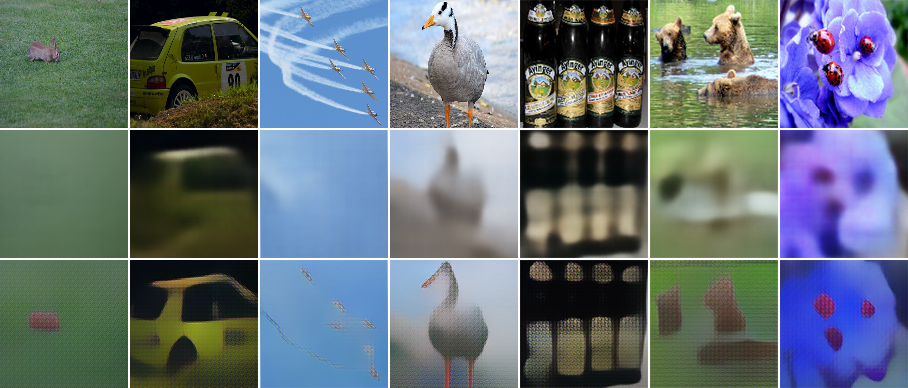
\includegraphics[width=0.8\linewidth]{bce_dfc_crop}\end{tikzfigure}}
  { \begin{tikzfigure}
      \centering
        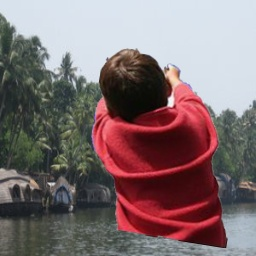
\includegraphics[width=0.195\linewidth]{syn1}
        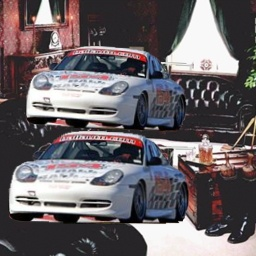
\includegraphics[width=0.195\linewidth]{syn2}
        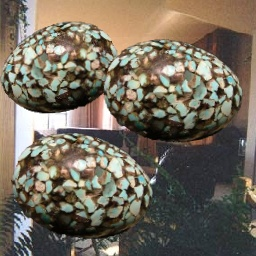
\includegraphics[width=0.195\linewidth]{syn3}
        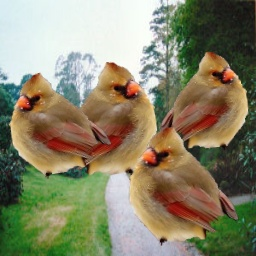
\includegraphics[width=0.195\linewidth]{syn4}
  \end{tikzfigure}
  }
\end{multicols}
}
\colorlet{innerblockbodybgcolor}{eccvgrayblue}

\useinnerblockstyle{eccvinner}
\innerblock{}{
\renewcommand{\columnseprulecolor}{\color[HTML]{FFFFFF}}
\setlength\columnsep{90pt}
\setlength\columnseprule{0.05cm}
%% \setlength\columnseprule{0.0cm}
\begin{multicols}{2}
{\boldblue{Feature Perceptual Loss.} In our experiments we observed difficulties with reconstructing multiple salient objects, negatively affecting the ability to subitize. Therefore, we employ the recent feature perceptual loss which uses intermediate layer representations in the objective function of the autoencoder.\par}
{A mixture of natural images and \boldblue{synthetic data} was used to augment the SOS dataset. Images are synthesized by cut-pasting objects onto natural image backgrounds. Subsequently, we apply random image transforms to each object to increase diversity in appearance. }
\vskip 0.11em
\end{multicols}
}
}

\useblockstyle{eccv2}
\begin{columns}
\column{0.435}
\block{SUBITIZING TASK PERFORMANCE}{
\colorlet{innerblockbodybgcolor}{white}
\innerblock{}{
\begin{tikzfigure}
    %% \begin{tabular*}{\innerblocklinewidth}{{\extracolsep{\fill}}lllllll}
    \begin{tabular}{lllllll}
    \toprule
    Count Label $\rightarrow$ & \quad 0 & \quad 1 & \quad 2 & \quad 3 & \quad 4+ & \quad mean \\
    \midrule
    %% \rowcolor
    Chance & \quad 27.5 & \quad46.5 & \quad18.6 & \quad11.7 & \quad\phantom{0}9.7 & \quad22.8 \\
    GIST & \quad 67.4 & \quad65.0 & \quad32.3 & \quad17.5 & \quad24.7 & \quad41.4 \\
    SIFT+IFV & \quad 83.0 & \quad68.1 & \quad35.1 & \quad26.6 & \quad38.1 & \quad50.1 \\
    CNN\_FT & \quad 93.6 & \quad93.8 & \quad75.2 & \quad58.6 & \quad71.6 & \quad78.6 \\
    VAE + softmax (ours) & \quad76.0 & \quad49.0 & \quad40.0 & \quad27.0 & \quad30.0 & \quad44.4 \\
    \bottomrule
    \end{tabular}
\end{tikzfigure}
}
\colorlet{innerblockbodybgcolor}{eccvgrayblue}
\innerblock{}{\boldblue{VAE + softmax.} \blindlist{enumerate}[2]}
}
\column{0.565}
%% \block{QUALITATIVE ANALYSIS}{
%% \colorlet{innerblockbodybgcolor}{white}
%% \innerblock{}{
%%   \begin{tikzfigure}
%%     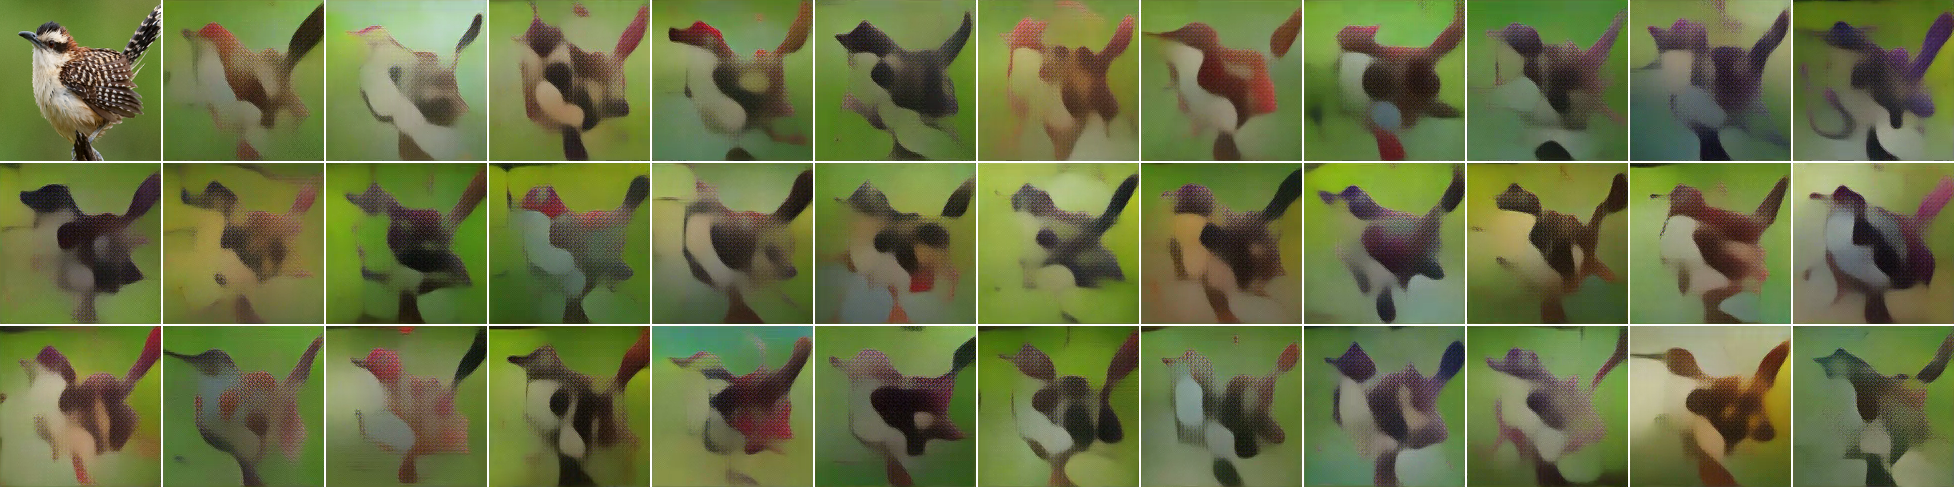
\includegraphics[width=35cm]{bird_varied_crop}
%%   \end{tikzfigure}
%% }
%% \colorlet{innerblockbodybgcolor}{eccvgrayblue}
%% \innerblock{}{
%%   \begin{tikzfigure}
%%     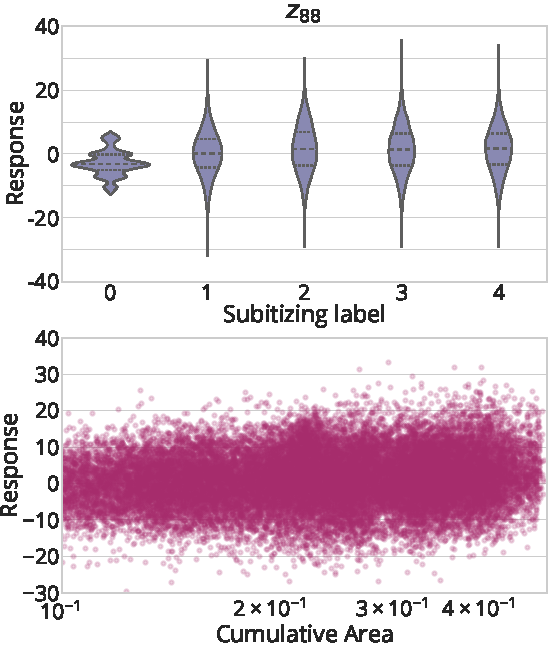
\includegraphics[width=18cm]{NA}
%%   \end{tikzfigure}
%% }
%% }
\end{columns}

%% \end{columns}

%% \begin{columns}
%% \column{0.6}
%% \block{Blocktile}{text}
%% \column{0.4}
%% \block{Blocktile}{text}
%% \end{columns}

\useblockstyle{reference}
% not sure if this actually centers text but it is more centered I guess
\block[bodyinnersep=12pt, bodyoffsetx=19pt]{}{\noindent\makebox[\linewidth]{\textcolor{lightgrey}{\rule{0.75\paperwidth}{0.12cm}}}
\begin{center}
\bibliography{poster}
\end{center}
}

\end{document}
